\chapter{相关工作}\label{chap:related_work}

本章主要介绍二进制翻译的相关工作,包括软硬协同二进制翻译器和纯软件二进制翻译器。
并对二进制翻译器的性能开销进行分析,发现间接跳转的性能开销以及指令集语义差异是二进制翻译器性能的主要瓶颈。
进而为了解决间接跳转的问题,引出了复杂指令集X86处理器的微码缓存的概念,为微译器的设计提供了设计思路。

\section{软硬协同二进制翻译器}

指令集作为软件和硬件沟通的桥梁,设计初衷是让软件和硬件设计解耦,使得软件开发者不需要关心硬件的细节,只需要关心软件的逻辑。
而二进制翻译器则是一种将不同指令集之间的桥梁,它可以将不同指令集的二进制代码翻译为目标指令集的二进制代码,从而实现不同指令集之间的兼容。
从设计层次来看,二进制翻译器相对指令集更加靠近硬件层,因此添加硬件支持的软硬协同二进制翻译器是一个比较自然的选择。

此外,二进制翻译器一般应用于生态迁移,在处理器厂商推出新型处理器时,为了保持对旧软件的兼容性,或者引入其他指令集已有的繁荣生态,需要引入二进制翻译器。
处理器厂商也有动力在新型处理器中添加硬件支持,以提高二进制翻译器的性能,减少软件兼容的性能开销。
本节主要介绍两个代表性的软硬协同二进制翻译器,分别是Transmeta公司的超长指令字兼容和龙芯公司的指令集扩展技术。

\subsection{超长指令字}

在处理器设计早期,由于当时的硬件晶体管资源有限,难以硬件发掘指令集并行性,因此超长指令字(Very Long Instruction Word, VLIW)技术应运而生。
超长指令字技术通过软件来发掘指令级并行性,将多条指令打包成一条超长指令字,从而提高指令级并行性,提高处理器的性能。
Transmeta公司推出的Crusoe处理器就是一种基于超长指令字的处理器,其宣称在性能和功耗方面都优于同期的X86处理器\cite{dehnertTransmetaCodeMorphing2003}。

但由于初期超长指令字技术的复杂性和软件开发者对于超长指令字的不熟悉,导致超长指令字生态并不繁荣,
因此Transmeta公司配套推出了软件上的代码转换器(Code Morphing Software, CMS),通过软硬协同的方式实现了对X86指令集的兼容。
Transmeta的CMS充当了翻译器和优化器的角色,使得基于非X86的VLIW处理器能够执行X86二进制代码。
还提供了一个动态优化的执行环境,能够在运行时对代码进行优化,从而提高执行效率和能耗性能\cite{dehnertTransmetaCodeMorphing2003}。

如图\ref{img:transmeta_arch}所示,代码转换器将从程序接收到的X86汇编代码指令翻译成微处理器的本机指令(超长指令字)。
通过这种方式,Crusoe 也可以模拟其他指令集架构,例如Crusoe 也能将字节码翻译为其本机指令集中的指令来执行 Java 字节码。

\begin{figure}[!htbp]
    \centering
    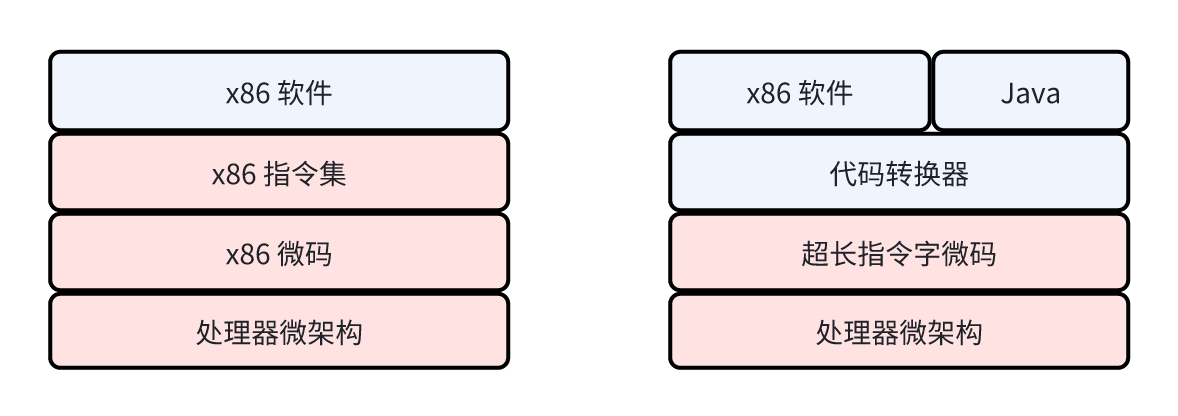
\includegraphics[width=0.8\linewidth]{./feishuImage/transmeta_arch.png}
    \caption{Transmeta架构图,在超长指令字处理器上实现兼容X86的指令集,并支持JAVA程序。}
    \label{img:transmeta_arch}
  \end{figure}
这种架构有如下特点:

\begin{itemize}
\item 架构兼容性与灵活性:Transmeta从初代128位VLIW处理器到第二代的256位VLIW处理器,都能通过软件翻译器保持软件兼容。
\item 解释与翻译配合:冷客户代码通过解释执行,热代码通过翻译执行,提高了执行效率。
\item 精确异常处理:Transmeta在硬件中引入了一套提交和回滚机制,当发生异常时,配合软件翻译器回滚,能够保证异常处理的精确性。
\end{itemize}

尽管Transmeta公司提出了许多创新的技术,但并未在市场上取得成功,最终于2007年退出处理器市场。
随着半导体工艺进步,处理器的晶体管资源变得丰富,基于硬件的乱序执行技术逐渐成熟,已经能够用硬件发掘指令级并行性,
超长指令字技术的优势逐渐减弱,超长指令字技术的发展也逐渐停滞。
但Transmeta公司在多架构兼容性方面的工作提供了宝贵的经验,成为软硬结合二进制翻译器的重要先驱者。

\subsection{指令集扩展}\label{sec:isa_extension}

客户和宿主指令集语义差异是二进制翻译器性能的主要瓶颈之一,为了解决这个问题,在宿主指令集中添加指令集扩展来接近客户指令集的语义是一种常见的解决办法。
例如龙芯公司在LoongArch指令中添加的二进制翻译扩展指令(Loongson Binary Translation, LBT)\cite{LoongArch2023}。

龙芯早期使用MIPS指令集,并添加了便于X86和ARM二进制翻译的一系列自定义指令集,例如对X86 EFLAGS的支持、对X87浮点指令的支持、非对齐访存的支持等,形成了LoongISA\cite{LoongISA}。
但由于MIPS中用户定义指令(UDI)槽位有限,导致了LoongISA的指令集扩展受限,
所以在2020年龙芯公司发布了全新的、自主可控的、支持更多指令集扩展的LoongArch架构\cite{LoongArch2023}。
并从3A5000开始,龙芯处理器开始支持LoongArch架构,并配套使用LATX二进制翻译器进行x86应用程序的翻译。
LoongArch指令集中同样增加了对二进制翻译的扩展指令集,称为LBT(Loongson Binary Translation)指令集,用于支持x86、ARM、MIPS的二进制翻译。
LBT扩展指令集与LATX软件配合使用,可以实现更高效的二进制翻译,提高了龙芯处理器的软件兼容性。

指令集扩展虽然能够接近客户指令集的语义,但这样会增加宿主指令集的复杂度,更加剧了指令集的历史包袱,同时添加指令集扩展也难以支持多种指令集的兼容。

\section{软件二进制翻译器}

软件二进制翻译器是一种通过软件实现的二进制翻译器,
它对硬件改动较小,能够在不同的硬件平台上运行,因此具有更好的可移植性和灵活性。
本节主要介绍一款开源的用户态二进制翻译器QEMU,以及三款商用级的用户态二进制翻译器,包括苹果公司的Rosetta2、华为公司的ExaGear、龙芯公司的LATX。
其中Rosetta2和LATX也有硬件支持,但主要还是依赖软件实现,因此归类为软件二进制翻译器。

\subsection{QEMU}

QEMU是一个广泛使用的开源多平台二进制翻译框架,特别在云计算环境中,它常和KVM一起使用,提供了一种高效的虚拟化解决方案。
QEMU同时支持系统态翻译和用户态翻译,本文主要关注用户态翻译部分,它允许在一个主机操作系统上模拟另一个操作系统的应用程序。

QEMU也同时支持多种架构,包括x86、ARM、RISCV等,使其成为开发跨平台应用程序的理想工具, 也可用于软件开发、测试以及安全研究。
如图\ref{img:qemu_arch},它通过将不同指令集的机器代码翻译成中间语言(IR,Intermediate Representation),再将IR翻译成宿主指令集,实现跨架构的兼容性。
这种设计使得QEMU能够处理多种指令集,为用户提供了一定的灵活性。然而,QEMU的性能仅能达到原生性能的13\%,这主要归因于双层翻译(客户代码翻译到IR,IR翻译到宿主代码)的性能损失。

\begin{figure}[!htbp]
  \centering
  \includegraphics[width=0.6\linewidth]{./image/qemu-IR.pdf}
  \caption{QEMU二进制翻译器架构图,能在宿主指令集机器上运行多种客户程序。}
  \label{img:qemu_arch}
\end{figure}

基于QEMU的优化主要旨在提高其性能和执行效率,例如中间代码优化\cite{LiNan2021}、基本块链接优化\cite{Hong2012HQEMUAM}、缓存管理\cite{FengYue2010}、Helper函数优化\cite{Wang2021}等。
以下给出两个优化示例,包括HQEMU的多线程并行翻译和执行,以及寄存器分配的优化。

HQEMU\cite{Hong2012HQEMUAM}是一个基于QEMU和LLVM构建的多线程和可重定向动态二进制翻译器。
这个项目的目标是通过利用多核处理器的并行处理能力来减轻DBT的开销,同时允许更复杂的优化技术的应用。
HQEMU通过在不同的线程上分别运行QEMU翻译器和LLVM优化器,从而实现了这一目标。
在一系列基准测试中,比如SPEC CPU2006,HQEMU在x86到x86-64的模拟中,相比于原始的QEMU性能提高了2.4倍至4倍。

在动态二进制翻译中,寄存器分配是提高翻译代码执行效率的关键。原始的QEMU在许多宿主机上将所有目标寄存器映射到内存,并仅将少数临时变量存储在宿主寄存器中。
这种方法并没有考虑相邻指令之间的依赖关系,导致即使在执行前一个指令时已经将一个客户寄存器的值加载到临时变量中,执行下一个指令时也需要再次从内存中重新加载该值。
为了解决这个问题,\cite{Hong2012HQEMUAM}提出了一个优化方法,其在两个或更多相邻指令执行中有效利用了临时变量,
从而减少了对内存的不必要访问。通过这种优化,基准测试显示可以实现10\%到20\%的速度提升。

尽管以上优化示例展示了通过改进QEMU的翻译过程和内部机制,可以提升QEMU的效率和性能,
但是改进后的性能仍然仅相当于原生性能的一小部分,这在一些对性能要求较高的应用场景下显得不够可用。


\subsection{Rosetta2}

Rosetta2 是苹果公司开发的商用二进制翻译系统,
通过支持预先编译(AOT)和即时编译(JIT)两种模式实现动静结合翻译,
预先翻译对性能影响大的代码,并把翻译后代码保存在磁盘上,而对于需要动态解析的代码,采用即时编译的方式进行翻译。
Rosetta2 主要针对64位的x86\_64指令集进行翻译,以适配苹果M1等ARM64处理器的架构。

Rosetta2 的核心目标是保证MacOS上的软件能够在ARM架构下运行,这要求对系统调用进行转换,以匹配基于ARM的MacOS版本。
由于x86和ARM指令集都采用小端法(little-endian),这简化了指令翻译过程,避免了复杂的字节序反转操作。
这一点与苹果过去从PowerPC(大端法,big-endian)切换到x86的过程不同,后者在转换时面临更多的挑战。

然而,x86(强内存序)与ARM(弱内存序)在内存一致性模型上的差异可能导致多线程软件运行结果出现差异,这是模拟x86的一个主要挑战\cite{Risotto}。
苹果通过在芯片内部额外实现一个Intel版本的强内存TSO模型,并通过后门开关在运行Rosetta2时切换到该内存模型,解决了这一问题。
硬件支持的内存模型有效的降低来并发程序翻译的性能开销,提高了Rosetta2的性能。

\subsection{ExaGear}

ExaGear是华为公司开发的动态二进制翻译软件,专为在基于自研的ARM鲲鹏服务器上运行而设计。
ARM服务器由于其能效比优势,逐渐在数据中心中得到广泛应用,但是由于软件生态的限制,一些只有x86版本的软件无法在ARM服务器上运行。
ExaGear通过将x86应用程序翻译为ARM指令集,使得这些软件能够在ARM服务器上运行。

ExaGear通过修改Linux的binfmt\_misc组件,使得系统能够识别并使用ExaGear作为x86应用程序的解析器,实现了在安装过程中的高效集成。
ExaGear主要包括两个关键组件:指令翻译引擎和x86运行环境。指令翻译引擎充当x86应用程序与ARM架构服务器之间的中间件,实现了在x86应用程序启动时的实时翻译功能。
这一过程对用户完全透明,确保了用户体验的一致性。x86运行环境为x86应用程序提供了必要的标准库、实用程序和配置文件,构建了一个完整的运行时环境。
此外ExaGear还通过Trace优化技术来减少分支数目,进而改善内存布局和局部性,减少间接跳转查找过程\cite{LvYandong2021}。

\subsection{LATX}

龙芯二进制翻译器(LATX)是龙芯公司开发的一款动态二进制翻译软件,用于在龙芯处理器(LoongArch架构)上运行x86架构的应用程序。
结合LATX和Wine\cite{amstadt1994wine}(一 个 操 作 系 统 API翻译软件,它可以用Linux的系统调用来模拟实现Windows的系统调用,从而实现在Linux/ x86上运行Windows/x86的应用程序),
用户可以在龙芯处理器上运行大量的x86应用程序,包括Windows应用程序,例如微信、WPS、部分游戏等。

如前文\ref{sec:isa_extension}节所示,通过添加龙芯二进制翻译扩展指令(LBT),LATX能生成出更接近X86语义的宿主指令,而无需用多条指令模拟。
此外,LATX 也添加了各类优化措施,例如X86 EFLAGS延迟计算、基本块链接、跨基本款反馈优化等,更多细节可以参考胡起的硕士论文\cite{HuQi2023}。

表\ref{tab:BTs} 对本节提到的4个主流的二进制翻译器进行了总结。

\begin{table}[!htbp]
  \centering
  \caption{主流二进制翻译器}
  \label{tab:BTs}
    \begin{tabular}{llll}
    \rowcolor[HTML]{FBE5D6} 
    二进制翻译器    & 公司   & 客户平台           & 宿主平台           \\
    QEMU      & 开源项目 & X86,ARM,RISCV等 & X86,ARM,RISCV等  \\
    ExaGear   & 华为   & X86            & ARM            \\
    Rosetta2  & 苹果   & X86            & ARM            \\
    LoongArch & 龙芯   & X86            & LoongArch      
    \end{tabular}
    \end{table}

\section{软件二进制翻译的性能开销分析}\label{sec:bt_overhead_all}

\subsection{理论分析}\label{sec:bt_overhead}

在进行性能分析之前,我们可以先对二进制翻译器的性能开销进行理论分析。
如图\ref{img:bt_overhead},二进制翻译的性能开销主要分为两类:指令集语义差异和二进制翻译器机制的开销。

指令集是计算机软件和硬件交互的接口,是定义了计算机的操作和数据的格式的一种规范。
指令包括操作码和操作数,操作码是指令的功能码,操作数是指令的操作对象。其中操作数按照操作对象可以分为立即数、寄存器、内存等。
\begin{itemize}
\item 操作码不同导致一条客户指令翻译成多条宿主指令。
\item 如果客户指令的立即数范围大于宿主指令的立即数范围,那么需要额外的指令来加载立即数。
\item 如果客户指令的寄存器数量大于宿主指令的寄存器数量,那么需要额外的指令来保存和恢复寄存器,也称为寄存器溢出。
\item 如果客户指令的内存访问模式复杂,那么需要额外的指令来计算内存地址。
\end{itemize}

而二进制翻译器机制的开销主要包括:
\begin{itemize}
\item 间接跳转的性能开销:间接跳转是指在程序运行时,通过读取寄存器的值来决定跳转到哪个地址。这种跳转方式在静态翻译时无法确定,因此需要在运行时查询哈希表来确定跳转地址。
\item 翻译开销:翻译开销是指动态二进制翻译器在翻译客户指令时产生的性能开销。这种开销主要包括指令翻译、基本块优化、基本块链接等。
\item 代码缓存维护: 二进制翻译器需要维护一个软件的代码缓存,用于存储翻译后的宿主指令。当缓存满时,需要进行缓存替换产生开销。
\end{itemize}


\begin{figure}[!htbp]
  \centering
  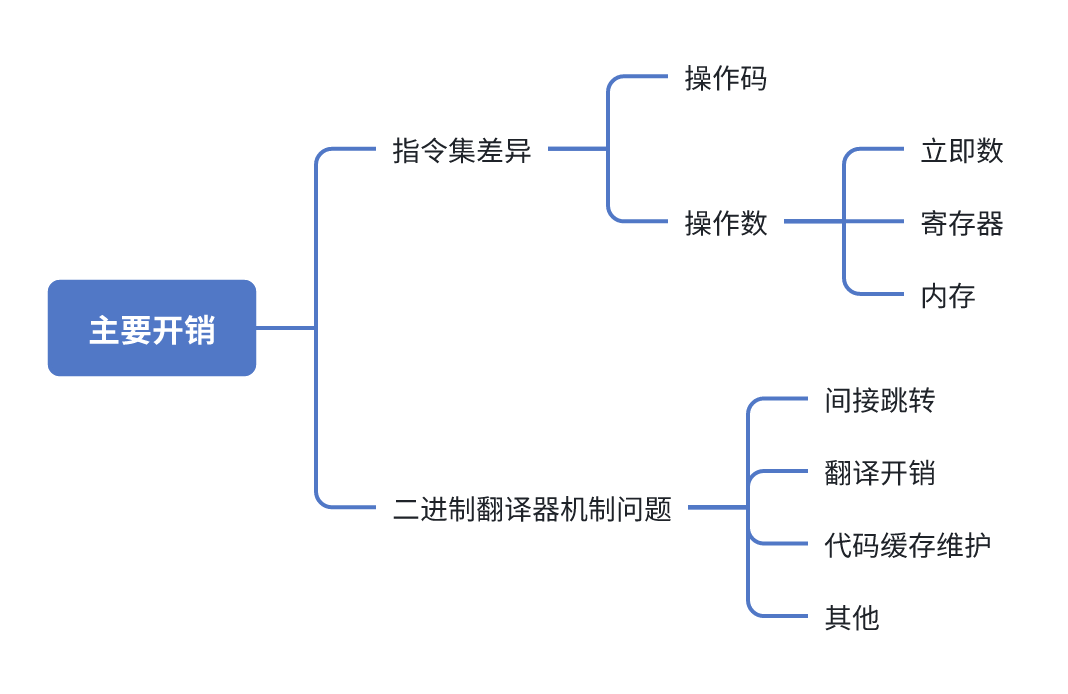
\includegraphics[width=0.7\linewidth]{./feishuImage/overhead.png}
  \caption{二进制翻译器的性能开销分析。}
  \label{img:bt_overhead}
\end{figure}

\subsection{实验分析}

上一节提到的商用级用户级二进制翻译器,例如苹果公司的Rosetta2(67.2\%)、华为公司的ExaGear(72.7\%)、龙芯公司的LATX(60\%)等,性能上仍然无法接近原生性能。
这些二进制翻译器采用一对一指令的翻译方式,即把一种指令集直接翻译到另一种指令集上(但一条客户指令可能翻译成多条宿主指令,产生指令膨胀,导致性能下降)。
它们虽然在理论上支持多架构翻译,但实际上需要投入较大的工程量,也可能造成性能下降。


\begin{figure}[!htbp]
  \centering
  \rotatebox{90}{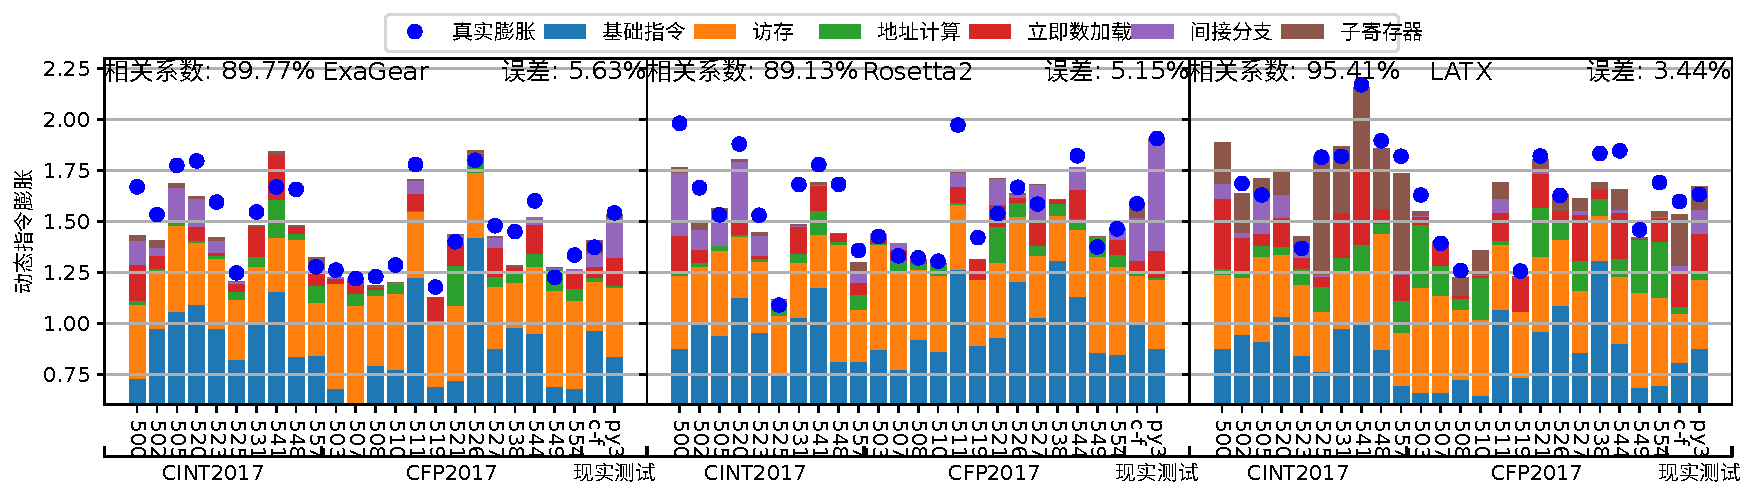
\includegraphics[width=\textheight,height=\textwidth,keepaspectratio]{./plot_pdf/insts_inflt_breakdown_2017.pdf}}
  \caption{各个二进制翻译器在运行SPEC2017的指令膨胀来源分析图。}
  \label{img:insts_inflt_breakdown_2017}
\end{figure}

根据我们之前完成的一项工作\cite{deflater},基于如下两个前提,我们使用使用指令膨胀率来分析二进制翻译器的性能开销。
\begin{enumerate}
\item  为了保证客户程序的精确异常,二进制翻译器不会做指令重排这样的激进优化,即保持指令的顺序不变。

\item  主流二进制翻译器在运行SPEC 2017这类运算密集型的基准测试时,98\%的时间都在执行生成的宿主指令上,而不是在翻译过程中。因此,我们认为翻译过程的性能开销是可以忽略不计的。

\end{enumerate}

指令膨胀率是指,每条客户指令平均翻译出的宿主指令数,是一个大于1的小数,计算方式参考\ref{eq:insts_inflt}。
举例来说,一条X86的add指令可能翻译成LoongArch的load指令和一个add指令,那么这条x86 add指令的膨胀率就是2。
对所有的客户指令的膨胀率求加权平均值,权重为客户指令的动态执行次数,即得到了整个程序的指令膨胀率
(为了说明简单,我们忽略了基本块内指令的优化)。
假设所有指令执行时间相同,那么膨胀了多少倍,程序的执行时间就会变长多少倍。
当然事实上,不同指令的执行时间是不同的,但是我们可以大致通过指令膨胀率来估计程序的性能开销。
指令膨胀率越高,翻译后的程序要执行的指令数越多,执行时间越长,性能越低。即便多发射处理器能在单拍内执行多条指令,缓解更多指令带来的性能开销,
但根据我们的测试数据,指令膨胀率和性能下降值是保持正相关的\cite{deflater}。

如图\ref{img:insts_inflt_breakdown_2017},
我们测量并模拟了3款商用级二进制翻译器(ExaGear、Rosetta2、LATX)在运行SPEC2017的指令膨胀率,模拟误差在5\%以内。
注意这三款翻译器都是复杂指令集(X86)到精简指令集(ARM/ LoongArch)的翻译器,这两类指令集语义差异较大,因此指令膨胀率较高。
图中\ref{img:insts_inflt_breakdown_2017}蓝色的点表示测量的真实膨胀率,而分解成不同颜色的柱状图表示模拟的膨胀率来源。
根据指令膨胀率的来源,我们主要把开销分成了5类:

\begin{equation}
  \text{总体膨胀} = \frac{\text{生成的宿主指令数}}{\text{客户指令数}} \\
  = \frac{\sum_i \text{指令频次}_i \times \text{指令膨胀率}_i}{\sum_i \text{指令频次}_i}
  \label{eq:insts_inflt}
\end{equation}


%latex 使用1. 2. 3. 来编号
\begin{enumerate}
  \item \textbf{指令集间操作码差异:} 不同指令集的操作码差异引起Eflags计算等操作的额外指令翻译,增加了指令膨胀率。此外LoongArch对于子寄存器默认符号扩展,X86/ARM默认零扩展。对应图\ref{img:insts_inflt_breakdown_2017}中\textcolor{Sepia}{\textbf{棕色}}部分。
  
  \item \textbf{操作数据模式不同:} 复杂指令集(X86)可以直接访问内存,而其他精简指令集只能操作寄存器,导致操作数模式不同。对应图\ref{img:insts_inflt_breakdown_2017}中\textcolor{orange}{\textbf{橙色}}部分。
  
  \item \textbf{地址计算不同:} 复杂地址计算方式(X86)与其他指令集的简单计算方式导致在翻译时需要额外指令。例如X86计算地址$addr = base + index * scale +disp$; 其他的大多为$addr = base + offset$。 对应图\ref{img:insts_inflt_breakdown_2017}中\textcolor{green}{\textbf{绿色}}部分。
  
  \item \textbf{立即数加载:} X86是变长指令集,支持编码64位立即数和32位地址偏移;而其他指令集均为定长指令集,立即数的编码空间有限。在翻译一条带有长立即数的指令时,需要额外的访存指令(从内存加载长立即数)或者是多条立即数加载指令(多个短立即数拼接成一个长立即数)。对应图\ref{img:insts_inflt_breakdown_2017}中\textcolor{red}{\textbf{红色}}部分。
  
  \item \textbf{间接跳转:} 客户指令地址到宿主指令地址是非线性的,而间接跳转的目标地址在运行时才能知道,需要额外的几条指令查询间接跳转哈希表,导致性能开销。对应图\ref{img:insts_inflt_breakdown_2017}中\textcolor{Purple}{\textbf{紫色}}部分。
  
\end{enumerate}

以上五类主要开销也对应于上一节\ref{sec:bt_overhead}理论分析的内容:
前4个属于指令集语义差异(操作数据模式不同也属于复杂指令集和精简指令集的差异,也可归为操作码不同),而间接跳转属于二进制翻译机制问题。
由于x86\_64通用寄存器只有16个,少于ARM/LoongArch的32个通用寄存器,所有没有寄存器溢出产生的开销。
而翻译开销和代码缓存维护的开销在现代高性能二进制翻译器中也是可以忽略不计的。


以上这5类主要开销很难通过软件优化来解决,需要借助硬件辅助的方式来解决。

为了消除软件二进制翻译器的性能开销,特别是在处理指令集语义差异方面的挑战,本文采用了硬件辅助的策略。其中,一些关键的工作包括:

1. 融合微码以缩小指令集语义差距: 针对指令集间操作码差异、操作数据模式不同以及地址计算不同等问题,我们尝试通过融合微码的方式,减小不同指令集之间的语义差距,从而降低翻译的开销。

2. 微码缓存的思路应用: 针对立即数加载和间接跳转的性能开销,我们借鉴了X86微码缓存的思想,将立即数放入微码缓存行中直接加载,用微码缓存直接查询非线性的地址空间映射,消除这两类开销。

接下来,将介绍与X86微码缓存相关的工作,探讨如何借助硬件辅助手段进一步优化软件二进制翻译器的性能。


% \section{X86 微码缓存的相关工作}
\section{X86处理器微码缓存}\label{sec:complex_isa}

X86 微码缓存是为了在 X86 CPU 后端实现超标量乱序执行并降低译码功耗而引入的关键组件\cite{solomonMicrooperationCachePower2001},如图\ref{img:front_end_ucache}。以下是关于 X86 微码缓存的主要工作和设计特点:

\begin{figure}[!htbp]
  \centering
  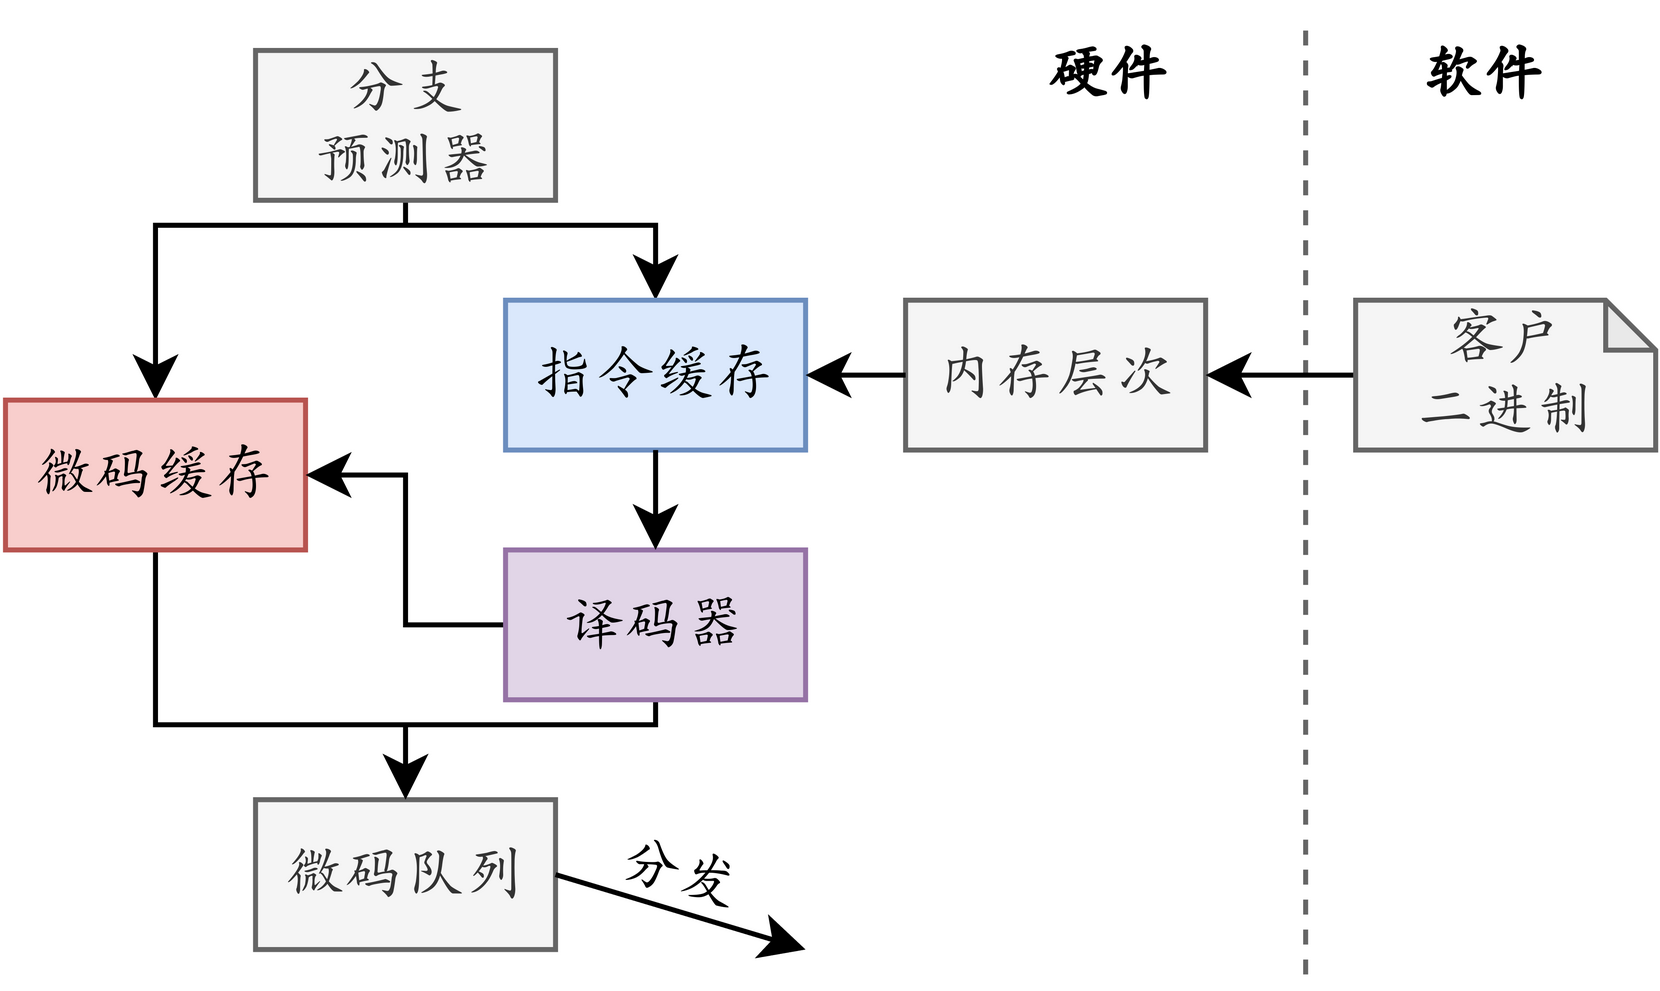
\includegraphics[width=0.8\linewidth]{./image/front_end_ucache.pdf}
  \caption{X86处理器前端架构图,包括指令缓存和微码缓存}
  \label{img:front_end_ucache}
\end{figure}


1. \textbf{微码与超标量乱序执行的关系:}

为了实现超标量乱序执行,X86 CPU 后端需要将复杂的变长x86指令转换成类RISC格式的定长微码。
微码的引入简化了指令集的关系,降低了CPU后端设计复杂度,使得指令能在后端能够更高效地乱序执行。

2. \textbf{微码缓存的引入:}

为了降低译码能耗、提高性能,研究者们引入了微码缓存,用于存储已经译码过的微码。
如果这条指令已经译码过,就直接从微码缓存中读取微码,而不需要再次译码。
\cite{solomonMicrooperationCachePower2001}论文中指出,在标准测试集中,
微码缓存能消除75\%的指令译码,在多媒体应用中,这个比例甚至高达90\%。
对于Intel P6处理器来说,能节省10\%左右的整机功耗。

3. \textbf{查询与缓存机制:}

具体而言,在CPU的前端,指令缓存和微码缓存是分开的,如图\ref{img:front_end_ucache}。
在前端译码阶段,系统会首先查询微码缓存,检查是否已经缓存了当前指令的微码。
如果微码已经在缓存中,CPU 就直接读取微码并发射到后端执行。
如果微码未缓存,系统则从指令缓存中取得指令,进行译码,并将译码结果存入微码缓存中,注意一个指令缓存行可能生成多个微码缓存行。

4. \textbf{缓存组织形式:}

\begin{figure}[!htbp]
  \centering
  \includegraphics[width=0.8\linewidth]{./image/ucache.pdf}
  \caption{微码缓存的组织形式}
  \label{img:ucache}
\end{figure}

微码缓存的组织形式与指令缓存有所区别。指令缓存的地址被分为标记、索引和块偏移三部分,而微码缓存的地址被分为标记、索引两部分,其中地址低位的块偏移也是标记的一部分。
这是因为一条指令会被译码为多条数量不定的微码,原本的块偏移无法唯一标识一条微码。
多条指令组成的指令基本块(以控制指令结尾)译码成的多条微码,会尽可能放在一个微码行中,然后用指令基本块的首地址来索引这个微码行。
同时一个指令缓存行产生的多个微码缓存行会放在同一个微码缓存组中,当需要刷新这一行指令缓存时, 可以方便的通过索引找到对应的微码缓存行进行刷新。
如图\ref{img:ucache},指令地址首先通过索引找到对应的微码组,然后通过标记找到对应的微码行。
微码行开头有元信息存储有关这个微码行的信息,例如微码数量、立即数数量等。接下来读出对应的微码,发射到后端执行。


5. \textbf{微码缓存行的结束条件:}

一行指令缓存可能对应多行微码缓存,这意味着当遇到指令缓存行结尾时,微码缓存会截断这一行,这样当一行指令缓存行需要刷新时,容易找到对应的多行微码缓存行进行刷新。
当遇到控制流指令时,微码缓存会截断这一行,确保每个微码缓存行只包含一个基本块的微码。
由于X86是变长指令集,微码是定长指令集,如果X86指令中有长立即数,会放在微码行的最后。
所以微码行中除了存入微码外,还会在最后存储立即数,见图\ref{img:ucache_line}。
微码和立即数是相向生长的,微码从前往后,立即数从后往前,如果相遇,说明微码行已满,需要分配新的微码行。

总结起来,微码缓存行有3个结束条件:1. 遇到指令缓存行的结尾;2. 遇到控制流指令并预测会跳转;3. 微码缓存行已满。

\begin{figure}[!htbp]
  \centering
  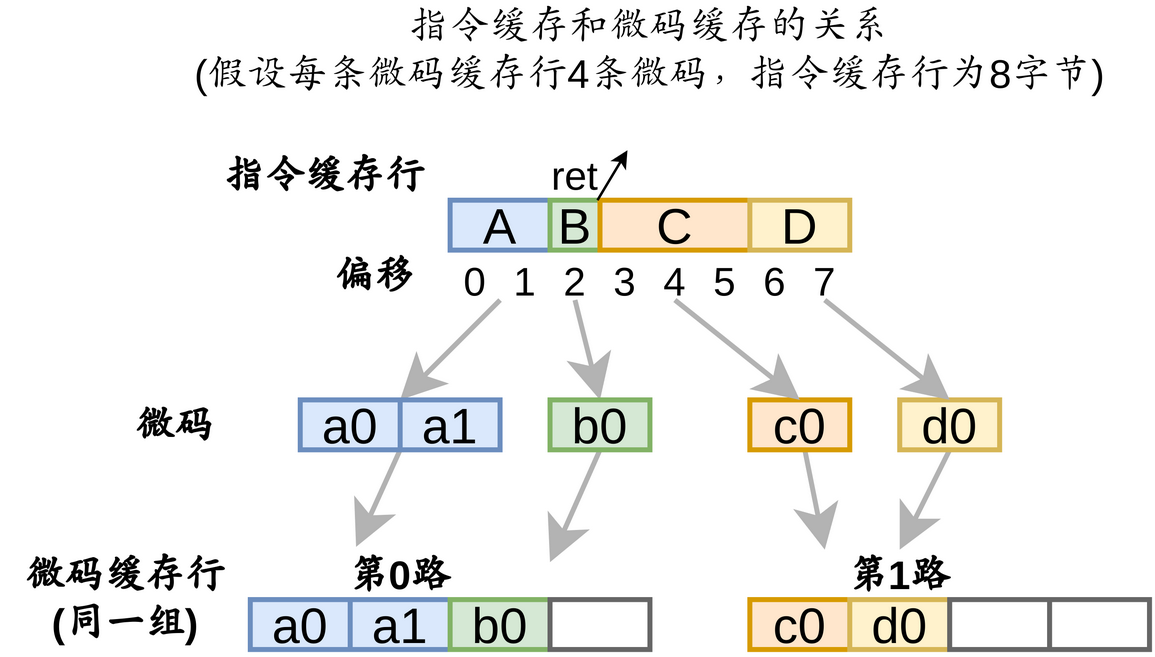
\includegraphics[width=0.8\linewidth]{./image/IC-to-UC.pdf}
  \caption{指令缓存和微码缓存关系}
  \label{img:IC_to_UC}
\end{figure}

如图\ref{img:IC_to_UC}给出了一行指令缓存对应多行微码缓存的示例(这里的微码行忽略了立即数的存储)。
假设指令缓存行为8字节,存储了A、B、C、D四条指令,分别长度为2、1、3、2字节,微码缓存行最多能存储4条微码。
A指令译码为的微码为a0,B指令的微码为b0,C指令的微码为c0,D指令的微码为d0。
则微码缓存行1存储了A指令的微码a0、a1和B指令的微码b0,微码缓存行2存储了C指令的微码c0和D指令的微码d0。
本来c0是可以存储在微码缓存行1中的,但是由于C指令是控制流ret指令,相当于指令A、B组成了一个基本块,C、D组成了另一个基本块,所以C指令的微码c0存储在微码缓存行2中。
此外微码缓存行1和微码缓存行2是存放在同一个微码缓存组中不同路上的,意味着它们的索引相同,但是标记不同。


X86 微码缓存的引入和优化为 X86 架构的超标量乱序执行提供了重要支持,使得 CPU 在执行 X86 指令集时能够更加高效地利用硬件资源,提高整体性能。

\begin{figure}[!htbp]
  \centering
  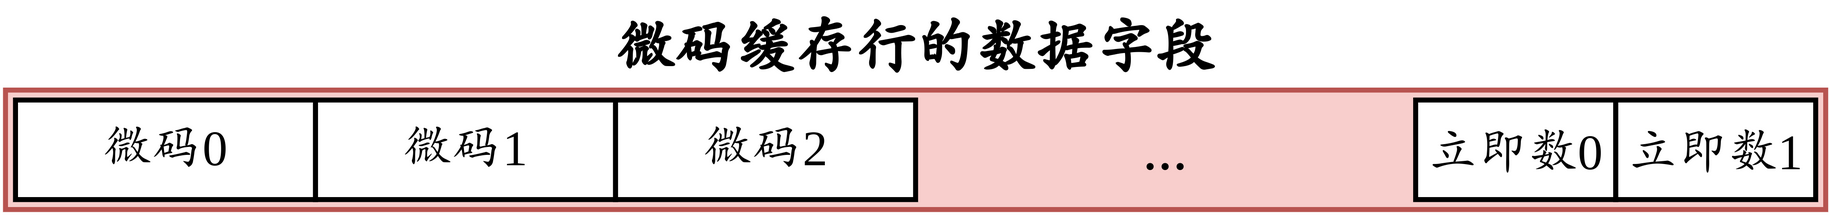
\includegraphics[width=0.8\linewidth]{./image/ucache_line.pdf}
  \caption{微码缓存一行的内容}
  \label{img:ucache_line}
\end{figure}
